%!TEX program = pdflatex
\documentclass[xcolor=dvipsnames, onlymath, 10pt, aspectratio=169, handout]{beamer}
\usecolortheme[named=Black]{structure}
% \usepackage{etex} % Too many packages
% \usepackage[utf8]{inputenc}
\usepackage[T1]{fontenc}
\usepackage{tipa}
\usepackage{color}
\usepackage{natbib}
\usepackage[french,english]{babel}
\usepackage{multicol}
\usepackage{caption}
\usepackage{vowel}
\usepackage{diagbox}
% \usepackage{fontawesome}
\usepackage{color}
\usepackage{tikz-qtree}
\usepackage{booktabs}
\usepackage{hyperref}
\usepackage{bibentry}
\usepackage{arydshln}
\usepackage{linguex}
\usetikzlibrary{arrows.meta, shapes, arrows, positioning, calc, trees}
\usepackage{pifont}
\usepackage{textgreek}
% \usepackage{eulervm}
\usepackage{libertinus}
\usepackage{inconsolata}
\usepackage{datetime}
% \setmonofont[Scale=0.85]{Berkeley Mono}
\definecolor{pastelorange}{RGB}{255,179,71}


% ============ >>>> MAC

\input{/Users/gdgarcia/Dropbox/Academia/LaTeX/garcia_latex_commands.tex}


% COURSE:

\newcommand{\course}{LNG-1100 : Méthodes expérimentales\\et analyse de données}

% TOPIC:

\newcommand{\classtopic}{\vspace{2ex}Intro : principes de base}

% DATE:

\newcommand{\classdate}{\fbox{1}}

% =====================================
% =====================================
% =====================================


% Define header colors:
\definecolor{lav1}{RGB}{184, 0, 35}
\definecolor{lav2}{RGB}{246, 195, 67}




\setbeamertemplate{itemize item}{$\bullet$}
\setbeamertemplate{itemize subitem}{$\circ$}
\setbeamerfont{frametitle}{series=\bfseries}
\setbeamercolor{frametitle}{fg=lav,bg=white}
\setbeamerfont{title}{series=\bfseries, parent=structure}
\setbeamercolor{title}{fg=lav,bg=white}



\usepackage[most]{tcolorbox}

    \tcbset{
        enhanced,
        colback=lavb!5!white,
        boxrule=0.1pt,
        colframe=lavb!80!white,
        fonttitle=\bfseries,
        width=5cm, box align=top,
        nobeforeafter
       }

\renewcommand\bibsection{\section[]{\refname}}
\usetheme{boxes}            % Simple and clear
\setbeamercolor{button}{bg=black,fg=white}
\beamertemplatenavigationsymbolsempty  % Remove nav controls




\title{\course}

\subtitle{\classtopic}

\author{Guilherme D.\ Garcia}


\institute[Université Laval] % (optional, but mostly needed)
{
  \mylink{https://fr.gdgarcia.ca}{fr.gdgarcia.ca}\vspace{5ex}
}


\date{\classdate}





\subject{Linguistique}


\begin{document}


\begin{frame}
	\vspace{2ex}
	\textcolor{lav1}{\noindent\rule{0.66\textwidth}{3pt}}
	\textcolor{lav2}{\noindent\rule{0.33\textwidth}{3pt}}

	\titlepage

	\vfill

	\begin{center}
		{\includegraphics[width=2.5cm]{/Users/gdgarcia/Dropbox/Academia/Admin/Uni-logos/ULaval1.png}}
	\end{center}

\end{frame}

\addtobeamertemplate{navigation symbols}{}{%
	\usebeamerfont{footline}%
	\usebeamercolor[fg]{footline}%
	\hspace{1em}%
	\vspace{1ex}%
	{\insertframenumber} sur {\inserttotalframenumber}
}



\setbeamertemplate{background}{\tikz[overlay,remember picture]\node[opacity=0.4, xshift=-1cm, yshift=.8cm] at (current page.south east){\includegraphics[width=.75cm]{/Users/gdgarcia/Dropbox/Academia/Admin/Uni-logos/ULaval2bw.png}};}

% ==================================
%  
%
% 
%    
%\end{frame}


\begin{frame}{Mesures d'accommodement}

	\begin{itemize}
		\item \lav{Important:}
		\item[] Les étudiants qui ont droit à des mesures d'accommodement en cours de session doivent procéder à leur activation immédiatement dans \mylink{https://monportail.ulaval.ca/accommodement}{monportail.ulaval.ca/accommodement} afin que celles-ci puissent être mises en place.

	\end{itemize}

\end{frame}


% ===============
%
% \begin{frame}{Mesures d'accommodement}
% 	\begin{itemize}
% 		\item[\winner] Si vous avez droit à des mesures d'accommodement, vous devez procéder à l'activation de celles-ci pour les cours et/ou les examens dans \mylink{https://monportail.ulaval.ca/accommodement}{monportail.ulaval.ca/accommodement} afin qu'elles puissent être mises en place
% 	\end{itemize}
% \end{frame}



% ===============


\begin{frame}{LNG-1100}{Objectifs}

	\begin{itemize}

		\item \textbf{Formuler et tester} des hypothèses de recherche [en linguistique]
		      %\begin{itemize} 
		      %	\item proposer des questions de recherche [pertinentes à la linguistique]
		      %	\item contraster des designs expérimentaux appropriés étant donnée une hypothèse spécifique 
		      %\end{itemize}

		      \pause

		\item \textbf{Se familiariser} avec les éléments de base de l’analyse de données quantitatives
		      %\begin{itemize}
		      %	\item manipuler des données en utilisant le langage R et l’extension tidyverse
		      %	\item décrire des patrons pertinents dans des données linguistiques en utilisant des tableaux et des figures
		      %	\item appliquer des modèles de régression aux données linguistiques
		      %\end{itemize}

		      \pause

		\item \textbf{Interpréter et synthétiser} des résultats statistiques dans un rapport scientifique
		      %\begin{itemize}
		      %	\item associer des résultats statistiques aux objectifs de recherche 
		      %	\item développer des rapports de recherche en utilisant Markdown et R
		      %\end{itemize}
	\end{itemize}

	\begin{importanttitle}{Nos analyses}
		\begin{itemize}
			\item Notre cours examine les données de façon \lav{quantitative}
			\item Une analyse \lav{qualitative} est également possible, bien qu'elle ne fasse pas partie de nos objectifs

		\end{itemize}
	\end{importanttitle}



\end{frame}

% ===============

\begin{frame}{LNG-1100}{Familiarisez-vous avec la structure du cours}

	\begin{center}
		\begin{tikzpicture}
			\Tree[.{\lav{LNG-1100}}
					[.monPortail [.Dates ] [.Évaluations ] [.Forum ] ]
					[.{\mylink{https://lng1100.quarto.pub/}{Livre numérique}} ]
					[.{\mylink{https://github.com/guilhermegarcia/LNG1100}{Dépôt Git}} [.Diapos ] [.Fichiers ] [.Données ] ]
			]
		\end{tikzpicture}
	\end{center}

\end{frame}


% ===============================

\begin{frame}{Nos matériels}

	\begin{itemize}
		\item[\winner] Livre du cours : {\mylink{https://lng1100.quarto.pub/}{lng1100.quarto.pub}} \smallCite{\citealt{garcia2023_lng1100}}
		\item[]
		\item Livres additionnels qui seront utilisés :

		\item[] \lav{Français} :
		      \begin{itemize}
			      \item[] \citet{barnier_R} \hfill introduction à R
			      \item[] \citet{larmarange2023} \hfill R + statistique
		      \end{itemize}

		\item[] \lav{Anglais} :
		      \begin{itemize}
			      \item \citet{wickham_rdata2023} \hfill R (très détaillé)
			      \item \citet{garcia_2021_dvaslr}\hfill R + statistique
		      \end{itemize}
	\end{itemize}

\end{frame}

% ===============================


\begin{frame}{Un petit sondage}{\mylink{https://forms.office.com/r/G700T82tNs}{forms.office.com/r/G700T82tNs}}

	\begin{center}
		
\includegraphics[width = 0.4\textwidth]{qr.png}
	\end{center}

\end{frame}

% ========================

\begin{frame}{Plan de la séance}

	\begin{enumerate}
		\item Les données peuvent être trompeuses
		\item Nos outils : \lav{R + RStudio}
		\item La structure du cours; principes généraux de la recherche (linguistique); hypothèse, expérimentation; comité d’éthique; design expérimental : sondage, ABX/AXB, tâche de jugement à choix forcé, etc.
	\end{enumerate}

\end{frame}

% ==================


\begin{transitionframe}


	Les données peuvent être trompeuses


\end{transitionframe}

% ==============================

\begin{frame}{Exemple 1}{Quel est le problème ici?}


	\begin{important}
		\begin{itemize}
			\item[] \textbf{Le chômage a baissé de 50 \% le mois dernier}
			      \pause
			\item[\winner] Si le taux de chômage est passé de 2 \% à 1 \%, c'est effectivement une baisse de 50\%, mais cela peut induire les gens en erreur en leur faisant penser qu'il y a eu une amélioration massive de l'emploi
		\end{itemize}
	\end{important}

\end{frame}

% ========================


% \begin{frame}{Exemple 2}{Quel est le problème ici?}
%
%
% 	\begin{important}
% 		\begin{itemize}
% 			\item[] \textbf{Notre produit est le plus en croissance sur le marché avec une augmentation des ventes de 200 \% le trimestre dernier}
% 			      \pause
% 			\item[\winner] Si le point de départ de cette croissance était un très faible nombre de ventes, l'augmentation en pourcentage peut sembler impressionnante, mais être trompeuse en termes de performance réelle sur le marché
% 		\end{itemize}
% 	\end{important}
%
% \end{frame}

% ========================

\begin{frame}{Exemple 2}{Quel est le problème ici?}


	\begin{important}
		\begin{itemize}
			\item[] \textbf{Le revenu moyen dans la ville A est de 100 000 \$}
			      \pause
			\item[\winner] Si un petit nombre de personnes très riches vivent dans la ville, la moyenne peut être fortement biaisée. La médiane ou le mode pourraient fournir un image plus précis du revenu typique
		\end{itemize}
	\end{important}

\end{frame}

% ========================

\begin{frame}{Exemple 3}{Quel est le problème ici?}


	\begin{important}
		\begin{itemize}
			\item[] \textbf{Le taux d'intérêt a augmenté de 2 \% l'année dernière}
			      \pause
			\item[\winner] Si le taux est passé de 5 \% à 7 \%, c'est une augmentation de 2 points de pourcentage, mais une augmentation de 40 \% du taux d'intérêt lui-même
		\end{itemize}
	\end{important}

\end{frame}


% ========================

\begin{frame}{Exemple 4}{Quel est le problème ici?}
	\label{maladie}
	\begin{important}
		\begin{itemize}
			\item[] \textbf{Un test médical avec une précision de 95 \% a donné un résultat positif. Par conséquent, le patient a 95 \% de chances d'avoir la maladie}
			      \pause
			\item[\winner] Sans tenir compte de la prévalence de la maladie dans la population, cette affirmation peut être trompeuse. Si la maladie est rare, un résultat positif peut toujours être un faux positif
		\end{itemize}
	\end{important}

	\only<2->{
		\begin{itemize}


			\item[] Pour bien comprendre le problème, on utilise \protect\myhyperdown{bayes}{le théorème de Bayes}

		\end{itemize}
	}

\end{frame}

% ===============

\begin{frame}{Exemple 5}{Quel est le problème ici?}

	\begin{itemize}
		\item Une figure peut-elle influencer vos conclusions?
		\item[]
	\end{itemize}

	\begin{center}
		\begin{figure}
			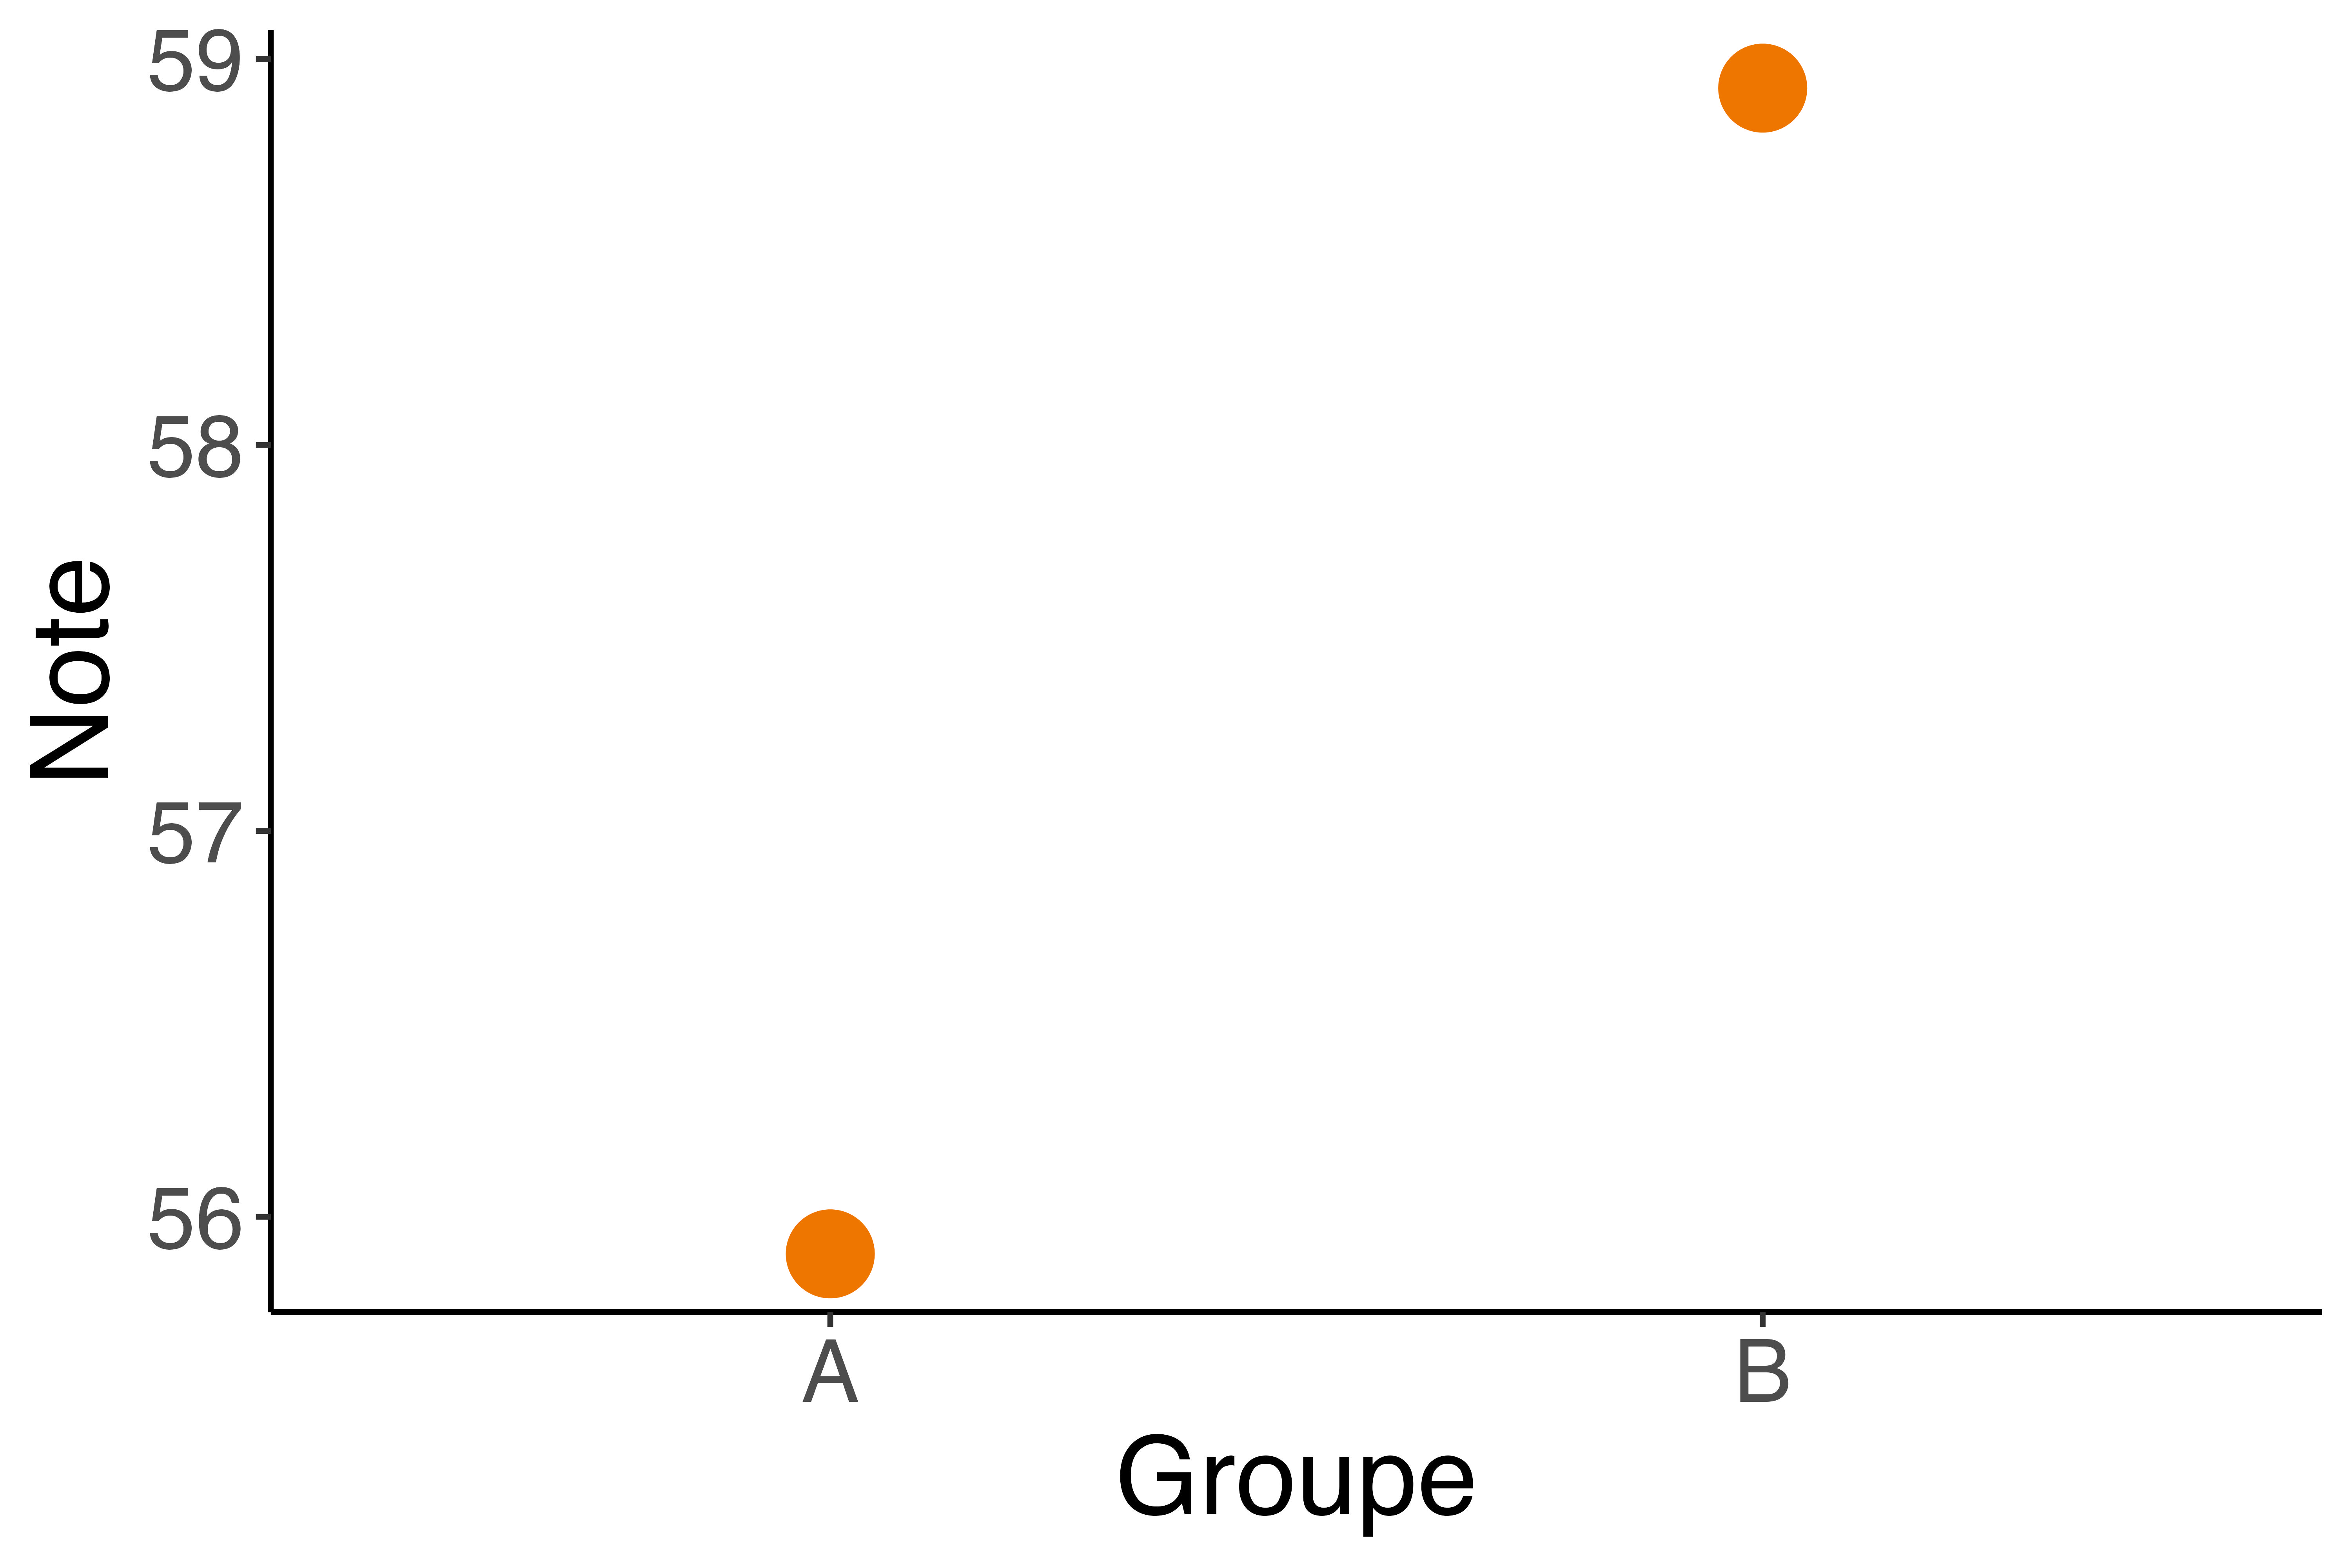
\includegraphics[width=0.45\textwidth]{1.jpeg}
			\pause
			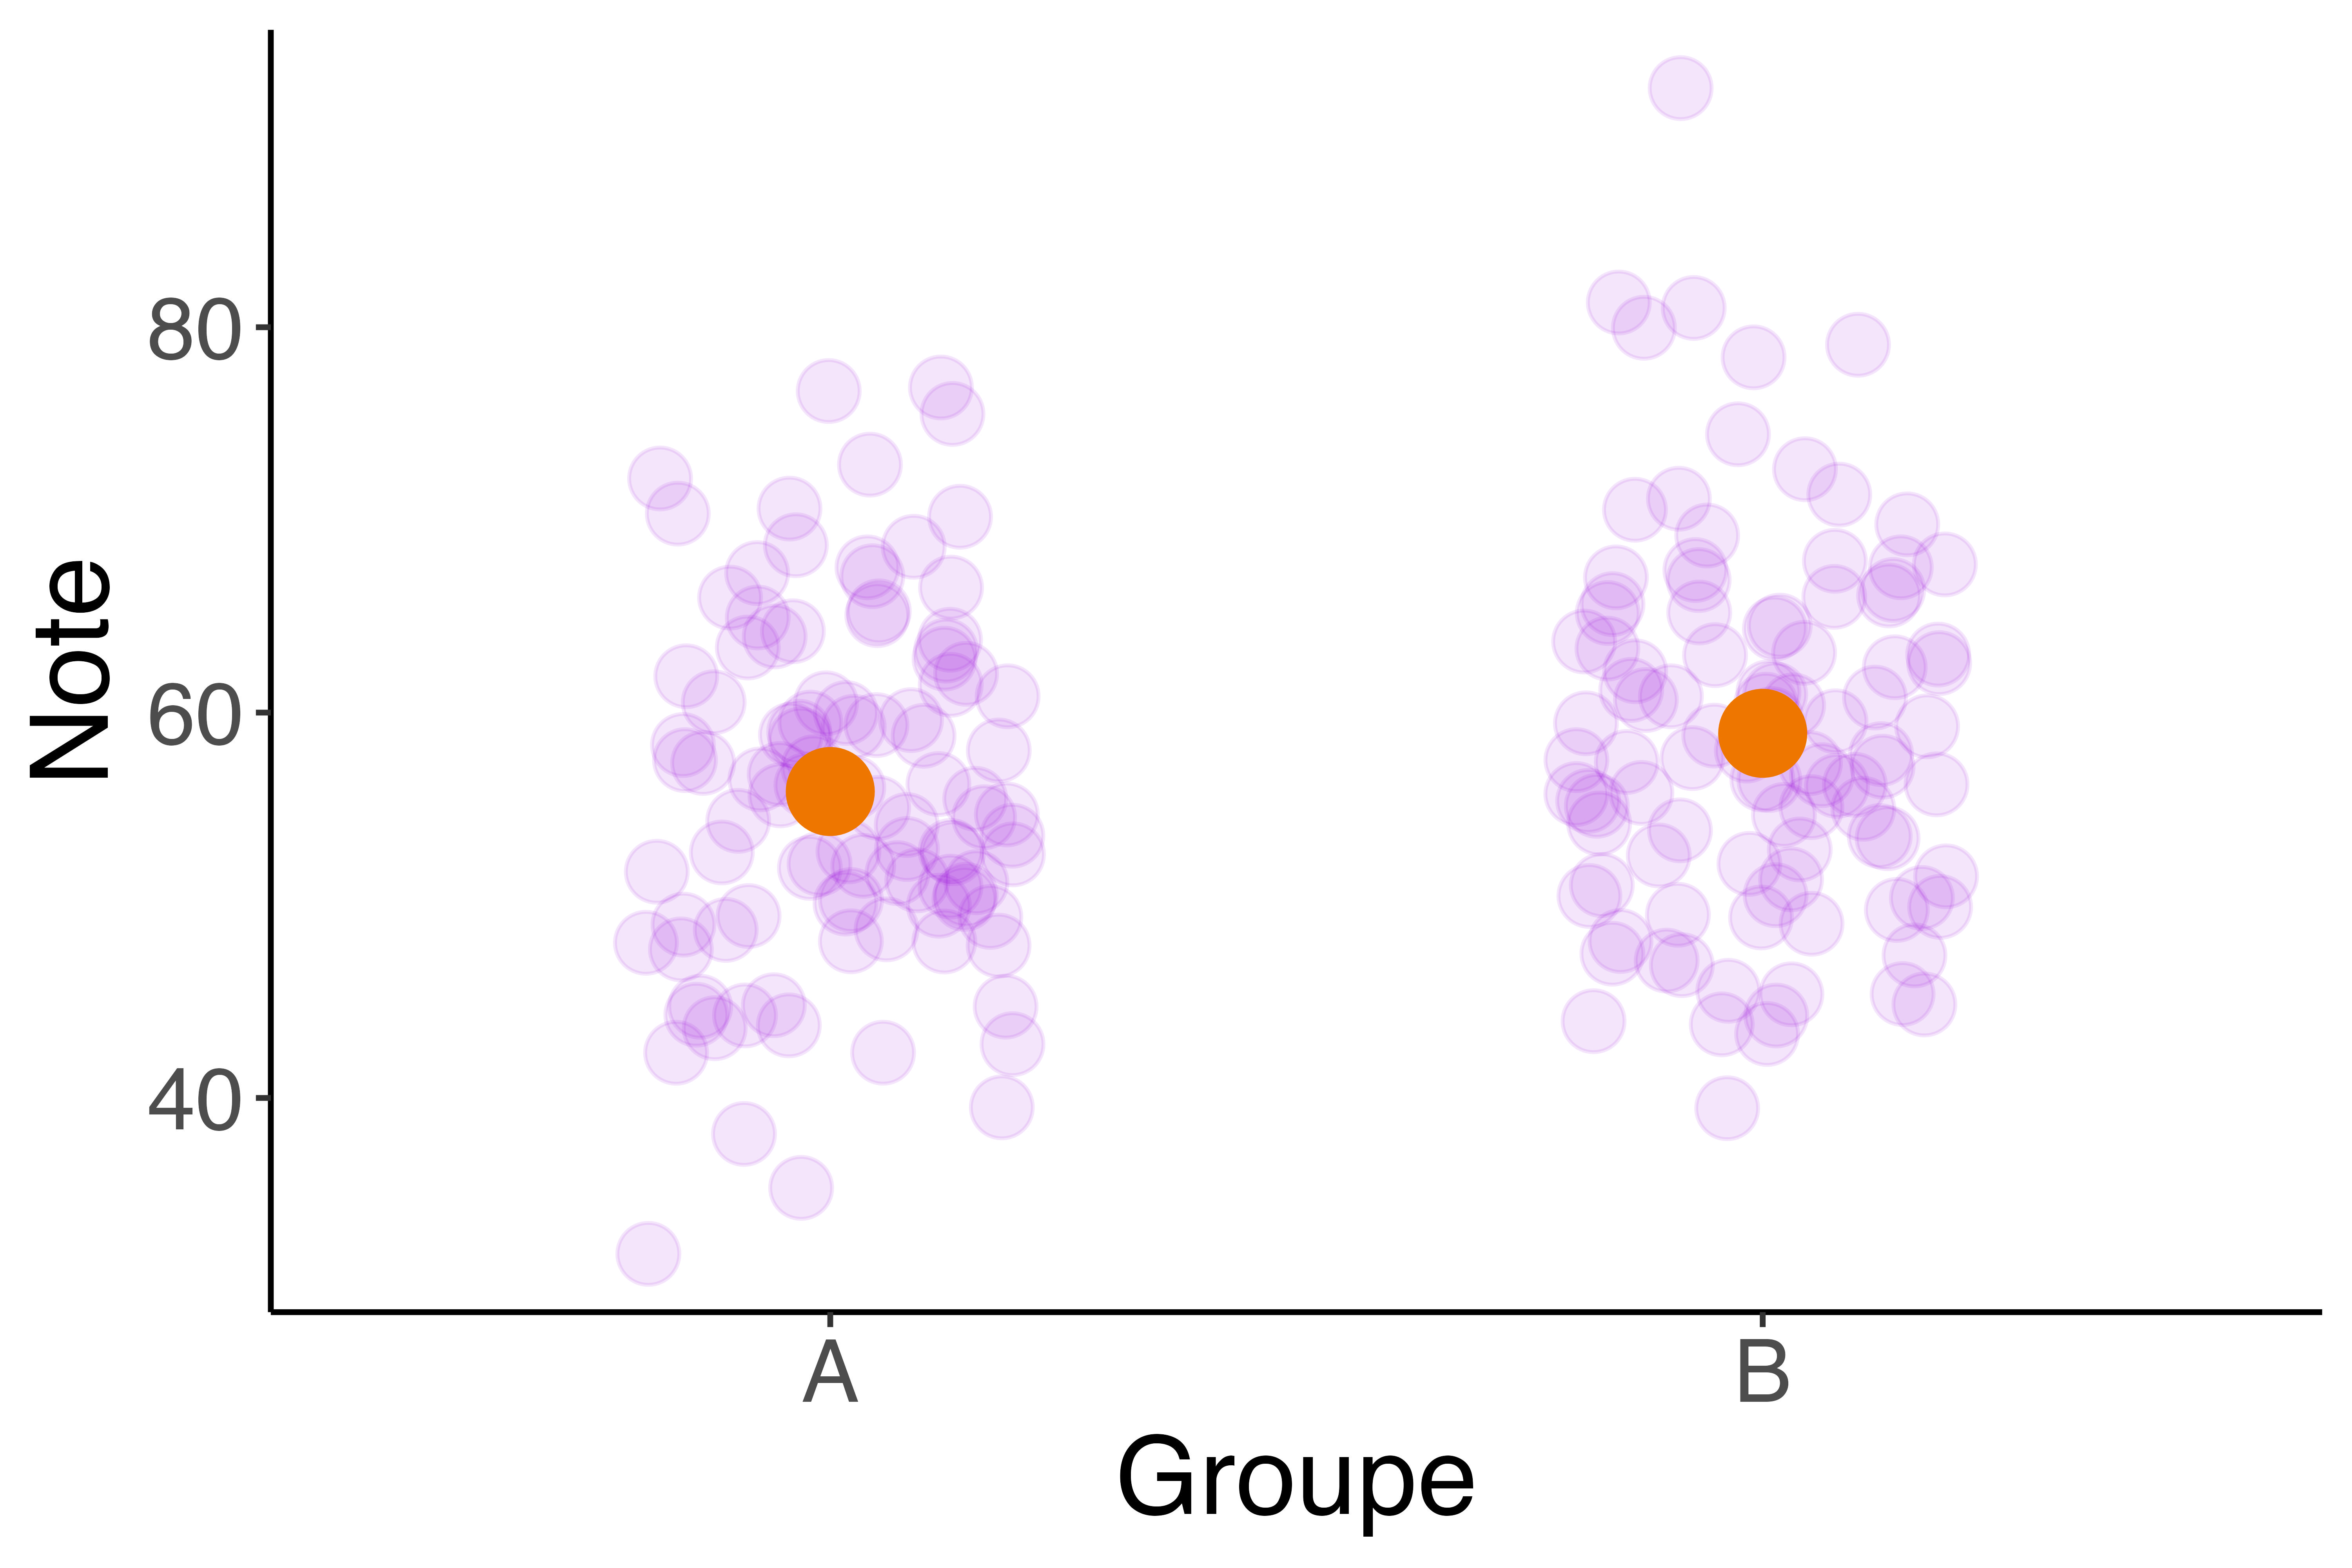
\includegraphics[width=0.45\textwidth]{2.jpeg}
		\end{figure}
	\end{center}

\end{frame}

% ===============


% ==================

\begin{frame}{Vos connaissances de base}{\mylink{https://forms.office.com/r/qqd8t6Tv1G}{forms.office.com/r/qqd8t6Tv1G}}

	\begin{center}
		
\includegraphics[width = 0.4\textwidth]{qr2.png}
	\end{center}


\end{frame}




% ==================

\begin{transitionframe}


	Nos outils : R + RStudio


\end{transitionframe}


% ========================

\begin{frame}{RStudio}

	\begin{itemize}
		\item On commence à travailler avec RStudio à partir de \textbf{la semaine prochaine}
		\item[\winner] Lisez le chapitre 1 de notre livre \lav{avant} notre séance
		\item[]
	\end{itemize}

	\pause

	\begin{center}
		\begin{tikzpicture}[->, scale = 0.8]
			\Tree[.{\lav{R} : langage + EDI\footnote{Environnement de développement intégré. Normalement, on choisit un EDI ou un éditeur de texte pour travailler avec le codage.} (+ ses \lav{extensions})}
					[.{\fbox{RStudio : l'EDI}}
							[.{Analyse de données} ]
							[.{Composition des documents} [.{Quarto} ] ]
					]
			]
		\end{tikzpicture}
	\end{center}

	\begin{itemize}
		\item Tous ces outils sont disponible dans la version en ligne \mylink{http://posit.cloud}{posit.cloud}
	\end{itemize}

\end{frame}

% ========================

\begin{frame}{R}{Langage + EDI simple}

	\begin{columns}[c]
		\begin{column}{0.7\textwidth}
			\begin{center}
				\includegraphics[width = .9\textwidth]{r-editor.png}
			\end{center}
		\end{column}
		%
		\begin{column}{0.3\textwidth}
			%\begin{center}
			
\includegraphics[width = 0.3\textwidth]{r.png}
			%\end{center}
			\begin{itemize}
				\item R inclut son propre EDI
				\item Mais il est trop simple
			\end{itemize}
		\end{column}
	\end{columns}


\end{frame}


% ==========



\begin{frame}{RStudio}{EDI très puissant et intuitif}

	\begin{columns}[c]
		\begin{column}{0.7\textwidth}
			\begin{center}
				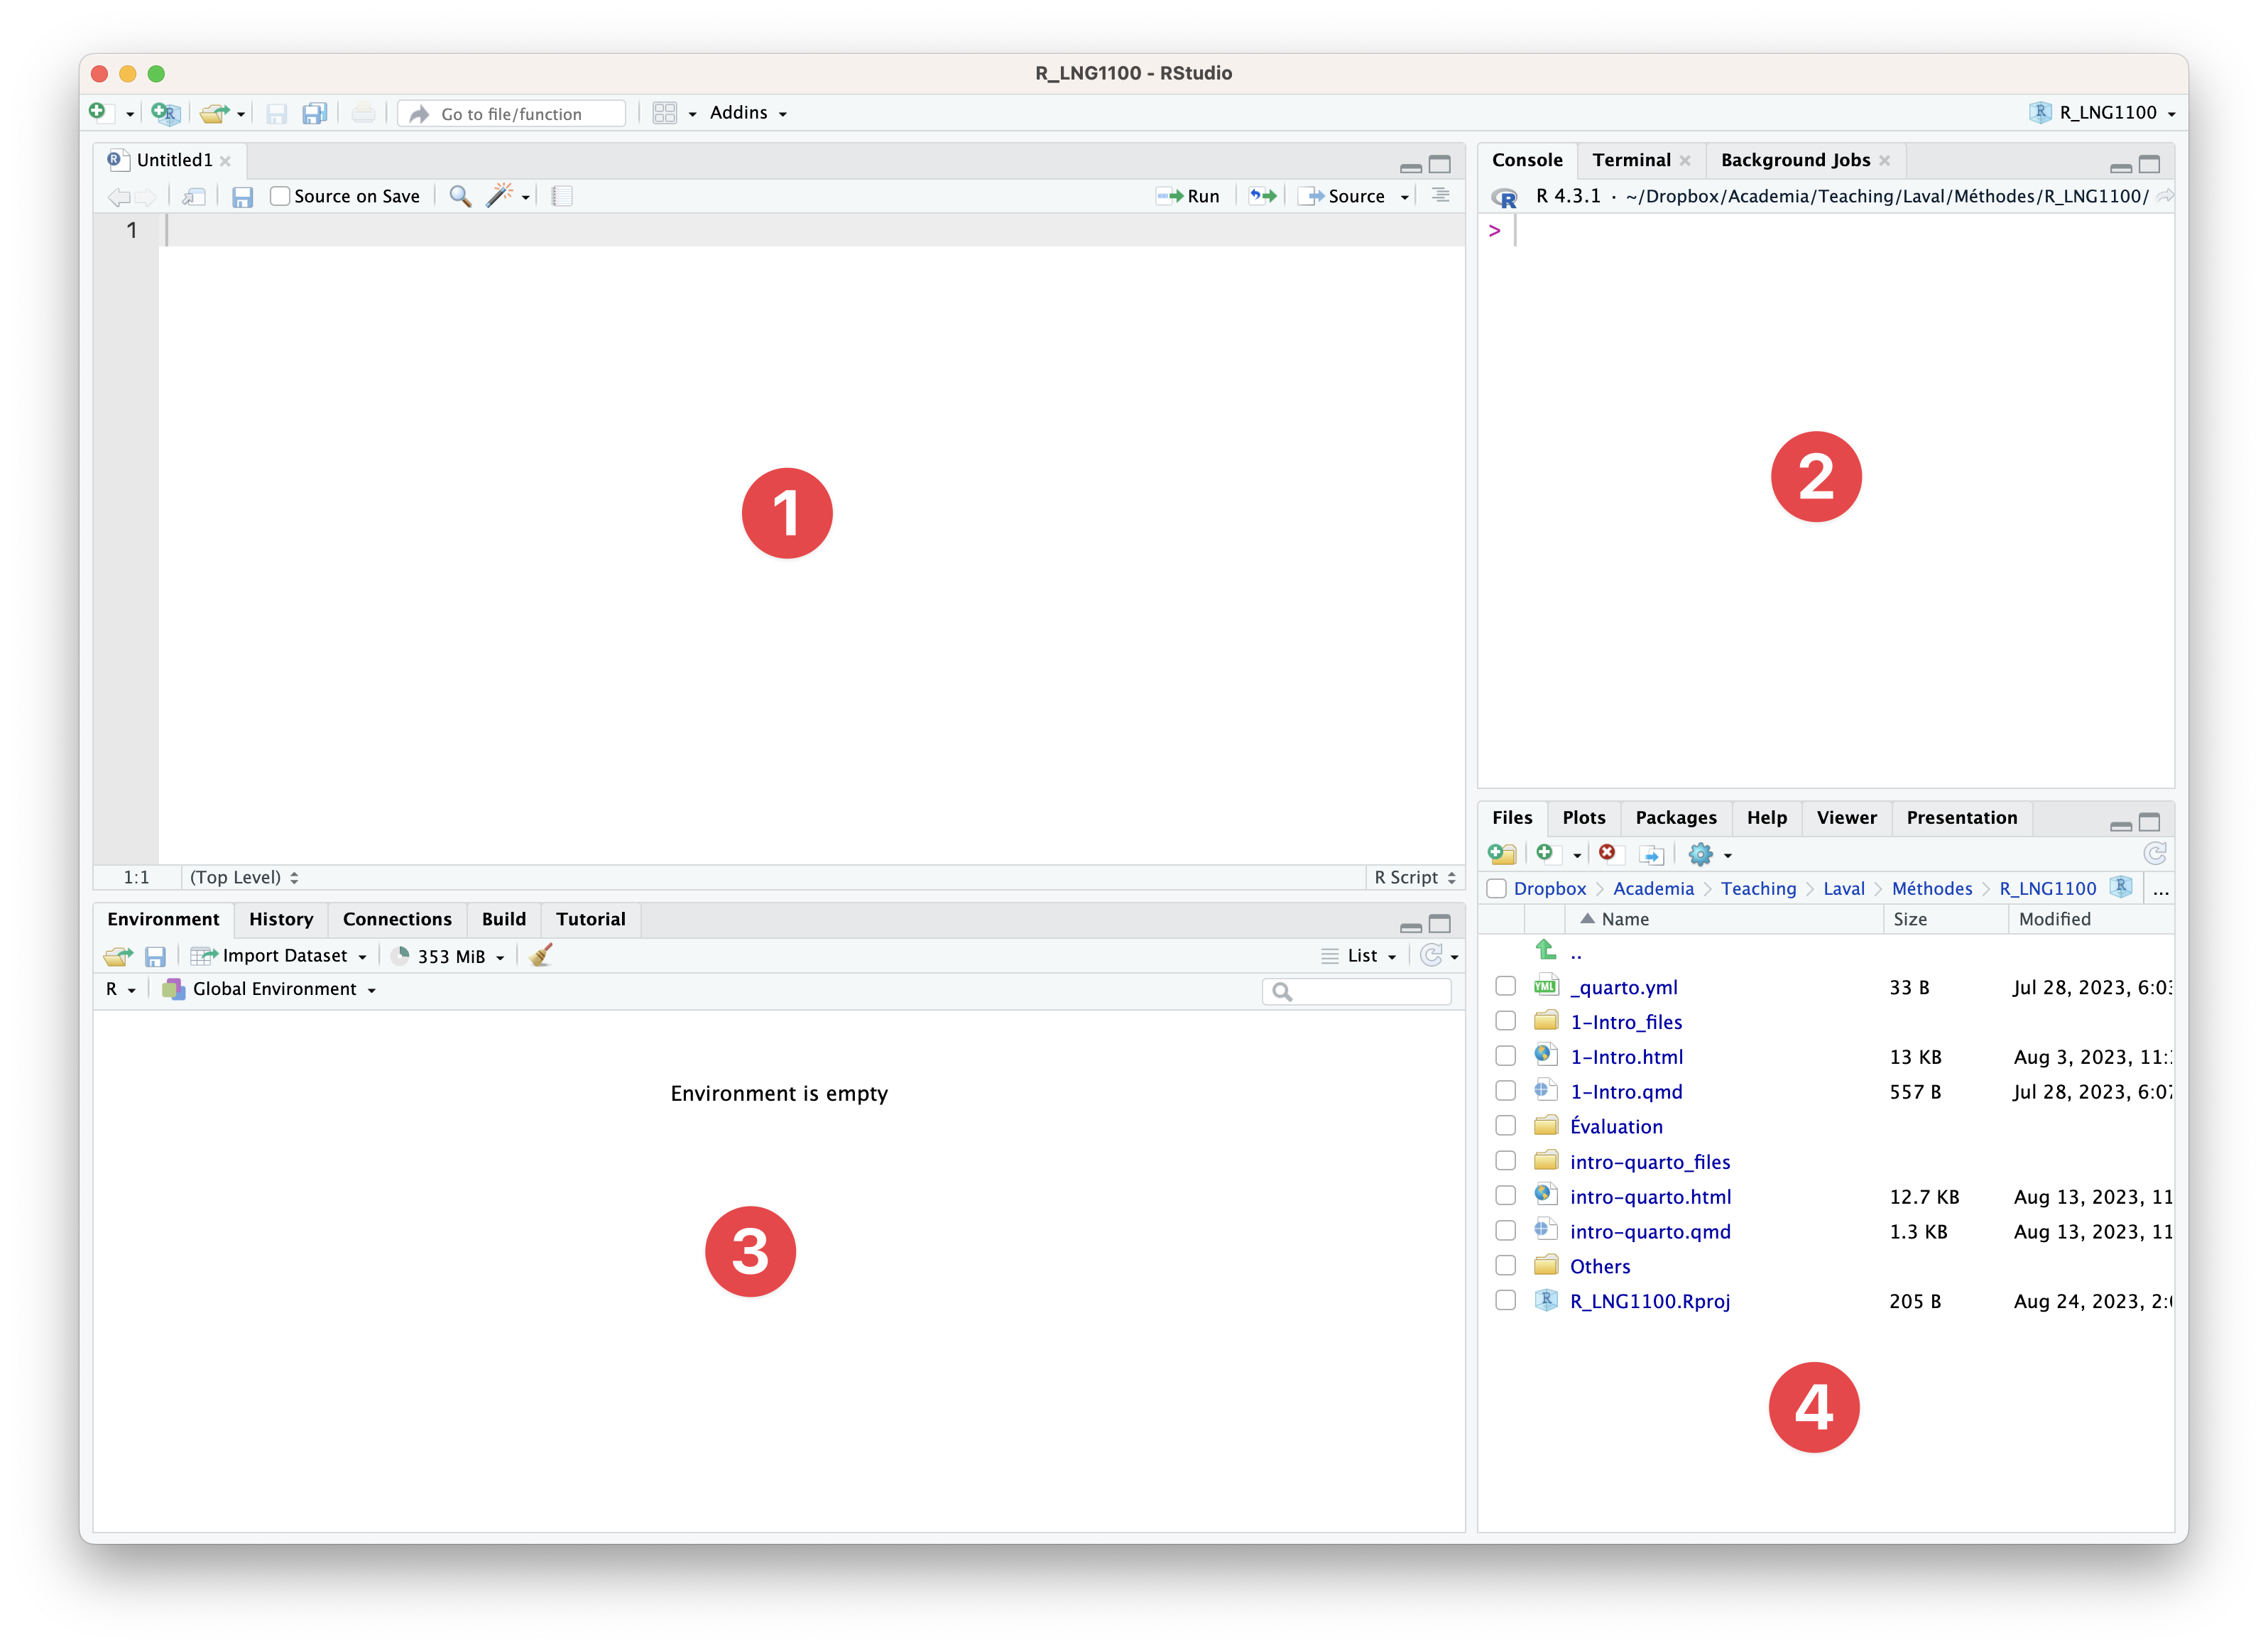
\includegraphics[width = 0.9\textwidth]{rstudio.png}
			\end{center}
		\end{column}
		%
		\begin{column}{0.3\textwidth}
			%\begin{center}
			
\includegraphics[width = 0.6\textwidth]{rstudio_logo.png}
			%\end{center}
			\begin{enumerate}
				\item Notre analyse
				\item Notre résultat
				\item Nos variables
				\item Fichiers locaux, figures
			\end{enumerate}
		\end{column}
	\end{columns}


\end{frame}


% ==========



\begin{frame}{Tidyverse}{Les extensions}

	\begin{itemize}
		\item Extension (\emph{package}) :
		\item[] collection de fonctions, de données et de documentation regroupées ensemble
		      \pause
		\item R contient plus de \textbf{17 000} extensions
		\item[\winner] Dans notre cours, on utilisera principalement l'extension \fbox{\var{tidyverse}}
	\end{itemize}

	\begin{center}
		
\includegraphics[width = 0.15\textwidth]{tidyverse.png}
	\end{center}

	\begin{itemize}
		\item On va explorer en détail \mylink{https://www.tidyverse.org/packages/}{cette famille d'extensions} dans deux semaines
	\end{itemize}

\end{frame}


% ==========
% ==================

\begin{transitionframe}

	Principes généraux de la recherche (linguistique)

\end{transitionframe}

% ==============


\begin{frame}{Le processus typique}

	\begin{enumerate}
		\item Trouver un sujet/problème approprié
		      \pause
		\item Poser une question\footnote{L'une des étapes les plus difficiles.} (et une hypothèse?)
		      \pause
		\item Développer une expérience et/ou \lav{collecter et examiner des données}
		      \pause
		\item \lav{Évaluer les résultats par rapport à l'hypothèse}
		      \pause
		\item \lav{Communiquer} et publier les résultats
	\end{enumerate}

	\vspace{3ex}

	\begin{itemize}
		\item[\winner] Dans notre cours, on met l'accent sur les éléments \lav{mis en évidence}
	\end{itemize}

\end{frame}

% ==========

\begin{frame}{Exemple}{Un sujet et une question de recherche}

	\begin{itemize}
		\item[1.] \textbf{Sujet} : la production et la perception des voyelles \ur{y {\o} \oe}\footnote{\mylink{https://fr.wikipedia.org/wiki/Alphabet_phon\%C3\%A9tique_international}{Alphabet phonétique international}} en français

		      \pause

		      \begin{itemize}
			      \item l\lav{u}nette - n\lav{eu}tre - j\lav{eu}ne $\leftarrow$ très difficile pour des apprenants
		      \end{itemize}

		      \pause

		\item[2.] Les apprenants qui prononcent mal ces voyelles sont-ils capables de les distinguer?% lorsqu'ils l'entendent?
		      \begin{itemize}
			      \item Si oui, il s'agit d'un problème de \lav{production}
			      \item Si non, ll s'agit d'un problème de \lav{perception} aussi
		      \end{itemize}
		      \pause

		\item[3.] On peut créer une expérience pour examiner le comportement des apprenants
		      \begin{itemize}
			      \item Par conséquent, il faut consulter le site du \mylink{https://www.cerul.ulaval.ca}{CÉRUL} (Comités d'éthique)
			      \item Parfois, le projet sera exempté (c'est rare...)
			      \item \textbf{Alternative} : utiliser des données déjà disponibles (p.\ ex., en ligne)
		      \end{itemize}
	\end{itemize}

\end{frame}

% ==========

\begin{frame}{Exemple}{Design expérimentale}

	\begin{itemize}
		\item Quel type de collecte de données...?
		      \begin{itemize}

			      \item Sondage (MS Forms et Google Forms : gratuits et faciles) $\leftarrow$ \red{Notre point de départ cette session}
			            \pause
			      \item ABX/AXB (PsychoPy, Gorilla, Praat, etc.)
			            \pause
			      \item Jugement à choix forcé (idem)
			      \item ...

		      \end{itemize}
	\end{itemize}

\end{frame}

% ==========

\begin{frame}{Exemple}{Design expérimentale : \fbox{sondage}}

	\begin{itemize}
		\item Le sondage est probablement le type de collecte de données le plus simple
		\item[\winner] Quel type de question pourrait-on poser dans un sondage sur les voyelles françaises?

		      \pause
		\item[]
		\item[] \fbox{\fr{Écoutez le mot suivant et tapez ce que vous entendez dans la casse ci-dessous}}
		\item[]

		      \pause

		\item On utilise plusieurs mots du français : ceux qui contiennent les voyelles ciblées et ceux qui contiennent d'autres voyelles (les \textbf{éléments distracteurs})
		\item[\winner] Enfin, on a de nombreuses réponses qui peuvent être analysées
	\end{itemize}

\end{frame}


% ==========

\begin{frame}{Exemple}{Design expérimentale : \fbox{ABX/AXB}}

	\begin{itemize}
		\item Méthode de comparaison entre deux stimulus
		\item Imaginons un mot non réel : `zule' \ur{zyl}

		      \pause
		\item Le participant écoute la séquence \ur{z\o l} - \ur{zyl} - \ur{zyl}
		\item[\winner] On pose la question :

		      \begin{itemize}
			      \item Le \lav{troisième} mot est-il identique au premier ou au deuxième mot? \fbox{1} \fbox{2} \hfill AB\lav{X}

			            \pause
			      \item Le \lav{deuxième} mot est-il identique au premier ou au troisième mot? \fbox{1} \fbox{3} \hfill A\lav{X}B
		      \end{itemize}

		      \pause

		\item Les réponses nous permettent d'évaluer la précision perceptuelle des participants

	\end{itemize}

\end{frame}

% ==========




\begin{frame}{Exemple}{Design expérimentale : \fbox{choix forcé}}

	\begin{itemize}
		\item On \textbf{force} le participant à choisir une option (entre deux/troix/etc.)

		      \pause
		\item Imaginons une paire minimale comme `peu' \ur{p\o} et `pu' \ur{py}

		      \pause
		\item Le participant écoute \ur{p\o}
		\item[\winner] On pose la question :

		      \begin{itemize}
			      \item Quel mot venez-vous d'écouter? \fbox{peu} \fbox{pu}
		      \end{itemize}


		\item Les réponses nous permettent d'évaluer la précision perceptuelle des participants

	\end{itemize}

\end{frame}

% ====================



\begin{frame}[t]{Design expérimentale}

	\begin{itemize}
		\item Supposons l'exemple ABX. On peut examiner plusieurs \lav{variables} d'intérêt :

		      \begin{itemize}
			      \pause
			      \item La voyelle (3 voyelles ciblées) et la précision de la réponse (0 ou 1)
			            \pause
			      \item Le temps de réaction pour chaque séquence
			      \item[]
			            \pause
			      \item Le niveau de compétence linguistique du participant
			            \pause
			      \item L'âge du participant
			      \item ...
		      \end{itemize}

		      \pause

		\item Finalement, on collecte aussi des données des locuteurs natifs (\textbf{groupe de contrôle}) pour s'assurer que l'expérience fonctionne
	\end{itemize}

	\begin{center}
		\begin{importanttitle}{Question}

			\begin{itemize}
				\item[\winner] Quel serait le problème si l’on ne collectait pas des données du groupe de contrôle?
			\end{itemize}


		\end{importanttitle}
	\end{center}

\end{frame}

% ==================

\begin{frame}{Exemples additionnels}{\fbox{ABX/AXB}}

	\begin{itemize}
		\item[] \fr{Écoutez les trois sons suivants : A, X, B. Le son \fbox{X} est-il plus semblable à A ou à B?}

	\end{itemize}

	\begin{center}
		\vfill
		\fbox{Exemple}
		\vfill
	\end{center}

\end{frame}

% ==========

\begin{frame}{Exemples additionnels}{\fbox{choix forcé}}


	\begin{itemize}
		\item[] {\textbf{\fr{Lequel de ces deux mots sonne plus naturel (en anglais)?}}}
		\item[]
	\end{itemize}
	\begin{center}
		{} [\ipaa{"kI.mE.s@r}] \hspace{3em} {} [\ipaa{kI."mE.s@r}]
	\end{center}


\end{frame}


% ====================


% =======================

\begin{frame}{Pratique}
	\begin{itemize}
		\item \lav{Question de recherche} : L'accent régional d'un locuteur influence-t-il la perception de son intelligence dans un contexte professionnel?

		\item \lav{Méthode} : une enquête où les participants écouteront des enregistrements de différents locuteurs avec différents accents régionaux présentant les mêmes informations professionnelles. Les participants devront ensuite évaluer l'intelligence perçue des locuteurs sur une échelle de 1 à 10.
	\end{itemize}


	\begin{important}
		\begin{enumerate}
			\item Quelles variables sont pertinentes dans l'étude en question?
			\item Quels sont les problèmes potentiels?
		\end{enumerate}
	\end{important}


\end{frame}

% ============


% ============

\begin{frame}{Méthodes $\rightarrow$ Analyse}{}

	\begin{itemize}
		\item Notre méthode de collecte de données détermine le type de données dans notre analyse :

		      \pause

		      \begin{itemize}
			      \item Temps de réaction = données continues $\rightarrow$ p.\ ex., \textbf{régression linéaire}
			            \pause

			      \item Choix forcé = données catégoriques (binaires) $\rightarrow$ p.\ ex., \textbf{régression logistique}
			            \pause

			      \item Échelle de classification = données scalaires $\rightarrow$ p.\ ex., \textbf{régression ordinale}
			      \item ...
		      \end{itemize}
		\item Il y toujours plusieurs méthodes appropriées d'analyse pour n'importe quel type de données
		\item[\winner] Par contre, on trouve aussi plusieurs choix d'analyse qui sont \lav{incorrects}

	\end{itemize}


\end{frame}



\begin{frame}[b]{Synthèse}



	\begin{center}

		\begin{tikzpicture}[->,>=stealth',shorten >=1pt,auto, scale=0.9,node distance=2.5cm,
				thick,main node/.style={rectangle,fill=lavy!20,draw,font=\sffamily\small}]

			% Define the nodes
			\node[main node] (0) at (0,1) {choisir le sujet};
			\node[main node] (1) at (0,-0.5) {poser la question};
			\node[main node, fill=lavb!20] (6) at (-3.5,-0.5) {\scriptsize hypothèse réfutable};
			\node[main node] (2) [below=of 1] {planifier la méthode};
			\node[main node] (3) [right=of 2] {analyser les données};
			\node[main node] (4) [above=of 3] {communiquer les résultats};
			\node[main node, fill=lavb!20] (5) at ($(3)!0.5!(4) + (3,0)$) {\scriptsize (Ré)évaluer la question(?)}; % between 3 and 4, to the right

			% Connect the nodes with arrows
			\draw[->] (0) -- (1);
			\draw[->] (1) -- (2);
			\draw[->] (2) -- (3);
			\draw[->] (3) -- (4);

			% Slightly curved arrows to and from the additional rectangle
			\draw[->, dashed] (3.north) to[out=0,in=180,looseness=1.2] (5.west);
			\draw[->, dashed] (5.north) to[out=180,in=0,looseness=1.2] (4.east);

			% Add a dashed, curved arrow
			\draw[->, dashed] (5) to[bend left=60] (2);
			\draw[<->, dashed] (6.east) -- (1.west);
		\end{tikzpicture}

	\end{center}
\end{frame}




% ============


\begin{frame}{Semaine prochaine}

	\begin{itemize}
		\item[]
		\item[\winner] Lisez attentivement les chapitres 1 et 2 de notre livre numérique
		\item Lisez \citet[ch.\ 1--3; 5--7]{barnier_R}
	\end{itemize}

\end{frame}






\appendix
\begin{frame}[allowframebreaks]

	{
		\footnotesize
		\frametitle{Références}
		\bibliographystyle{apalike}

		\bibliography{../../../../Dropbox/Academia/References/references}
	}

\end{frame}



%%%%%%%%%%%%%%%%%%%%%%%%%% APPENDIX

%%%%%%%%%%%%%%%%%%%%%%%%%%%%%%%%%%%%%%%%%%%%%%%%

\appendix


\begin{frame}
	\frametitle{Théorème de Bayes et tests médicaux}
	\framesubtitle{Informations additionnelles}
	\label{bayes}

	\begin{itemize}
		\item \textbf{On ne va pas étudier ce théorème ce semestre. Mais si vous êtes curieux :}
		\item[]
		\item[]   On considère un test avec une précision de \(95\%\), et une maladie rare (\(\frac{1}{1000}\)).
		      Quelle est la probabilité d'avoir la maladie si le résultat du test est \textbf{positif} ?

	\end{itemize}


	\vfill
	\vfill

	\myhyperup{maladie}{{Retourner}}

\end{frame}


% =============


\begin{frame}
	\frametitle{Définition des Probabilités}

	\begin{itemize}
		\item La probabilité d'avoir la maladie $P(M)$:
	\end{itemize}

	\begin{align*}
		P(M)        & = \frac{1}{1000}              \\
		P(\neg M)   & = 1 - P(M) = \frac{999}{1000} \\
		P(+|M)      & = 0,95                        \\
		P(+|\neg M) & = 0,05
	\end{align*}

	\vfill
	\vfill

	\myhyperup{maladie}{{Retourner}}


\end{frame}

% ======================

\begin{frame}
	\frametitle{Théorème de Bayes}

	Le théorème de Bayes :

	\begin{align*}
		P(M|+)     & = \frac{P(+|M) \times P(M)}{\lav{P(+)}}                     \\
		\lav{P(+)} & = P(+|M) \times P(M) + P(+|\neg M) \times P(\neg M)         \\
		           & = 0,95 \times \frac{1}{1000} + 0,05 \times \frac{999}{1000} \\
		           & = 0,0509                                                    \\
		P(M|+)     & = \frac{0,95 \times \frac{1}{1000}}{0,0509}                 \\
		           & \boxed{\approx 1,87\%}
	\end{align*}

	\vfill
	\vfill

	\myhyperup{maladie}{{Retourner}}


\end{frame}


% =============

\begin{frame}
	\frametitle{Théorème de Bayes}

	Le théorème de Bayes est formulé comme suit :

	\begin{align*}
		\text{Probabilité a posteriori} & : P(M|+)                                                                                         \\
		                                & = \frac{\text{Vraisemblance} \times \text{Probabilité a priori}}{\text{Vraisemblance marginale}} \\
		                                & = \frac{P(+|M) \times P(M)}{P(+)}                                                                \\
		                                & = \frac{P(+|M) \times P(M)}{P(+|M) \times P(M) + P(+|\neg M) \times P(\neg M)}
	\end{align*}

	Où \( P(M) \) est la probabilité a priori de la maladie, \( P(+|M) \) est la vraisemblance du test positif sachant la maladie, et \( P(+) \) est la vraisemblance marginale d'un test positif.


	\vfill
	\vfill

	\myhyperup{maladie}{{Retourner}}


\end{frame}

% =============

\end{document}
